\documentclass[10pt,xcolor={usenames,dvipsnames}]{beamer}

\usetheme[progressbar=frametitle]{metropolis}

\usepackage{booktabs}
\usepackage[scale=2]{ccicons}
\usepackage[geometry]{ifsym}
\usepackage{pgfplots}
\usepackage{multirow}
\usepgfplotslibrary{dateplot}
\usepackage[backend=biber,style=numeric-comp,sorting=none]{biblatex}

\usepackage{xspace}
\newcommand{\themename}{\textbf{\textsc{metropolis}}\xspace}
\graphicspath{{images/},{figures/}}
\addbibresource{Bibliografia/referencias.bib}




\title{Analisis estadistico del flujo de 1-gramas entre lenguajes indoeuropeos}
%\subtitle{And all that jazz}
\date{\today}
\author{Josué Ely Molina Becerra}
\institute{Universidad Nacional Autónoma de México
\\ \textbf{Asesor de tesis: Dr. Carlos Francisco Pineda Zorrilla}}
\titlegraphic{\hfill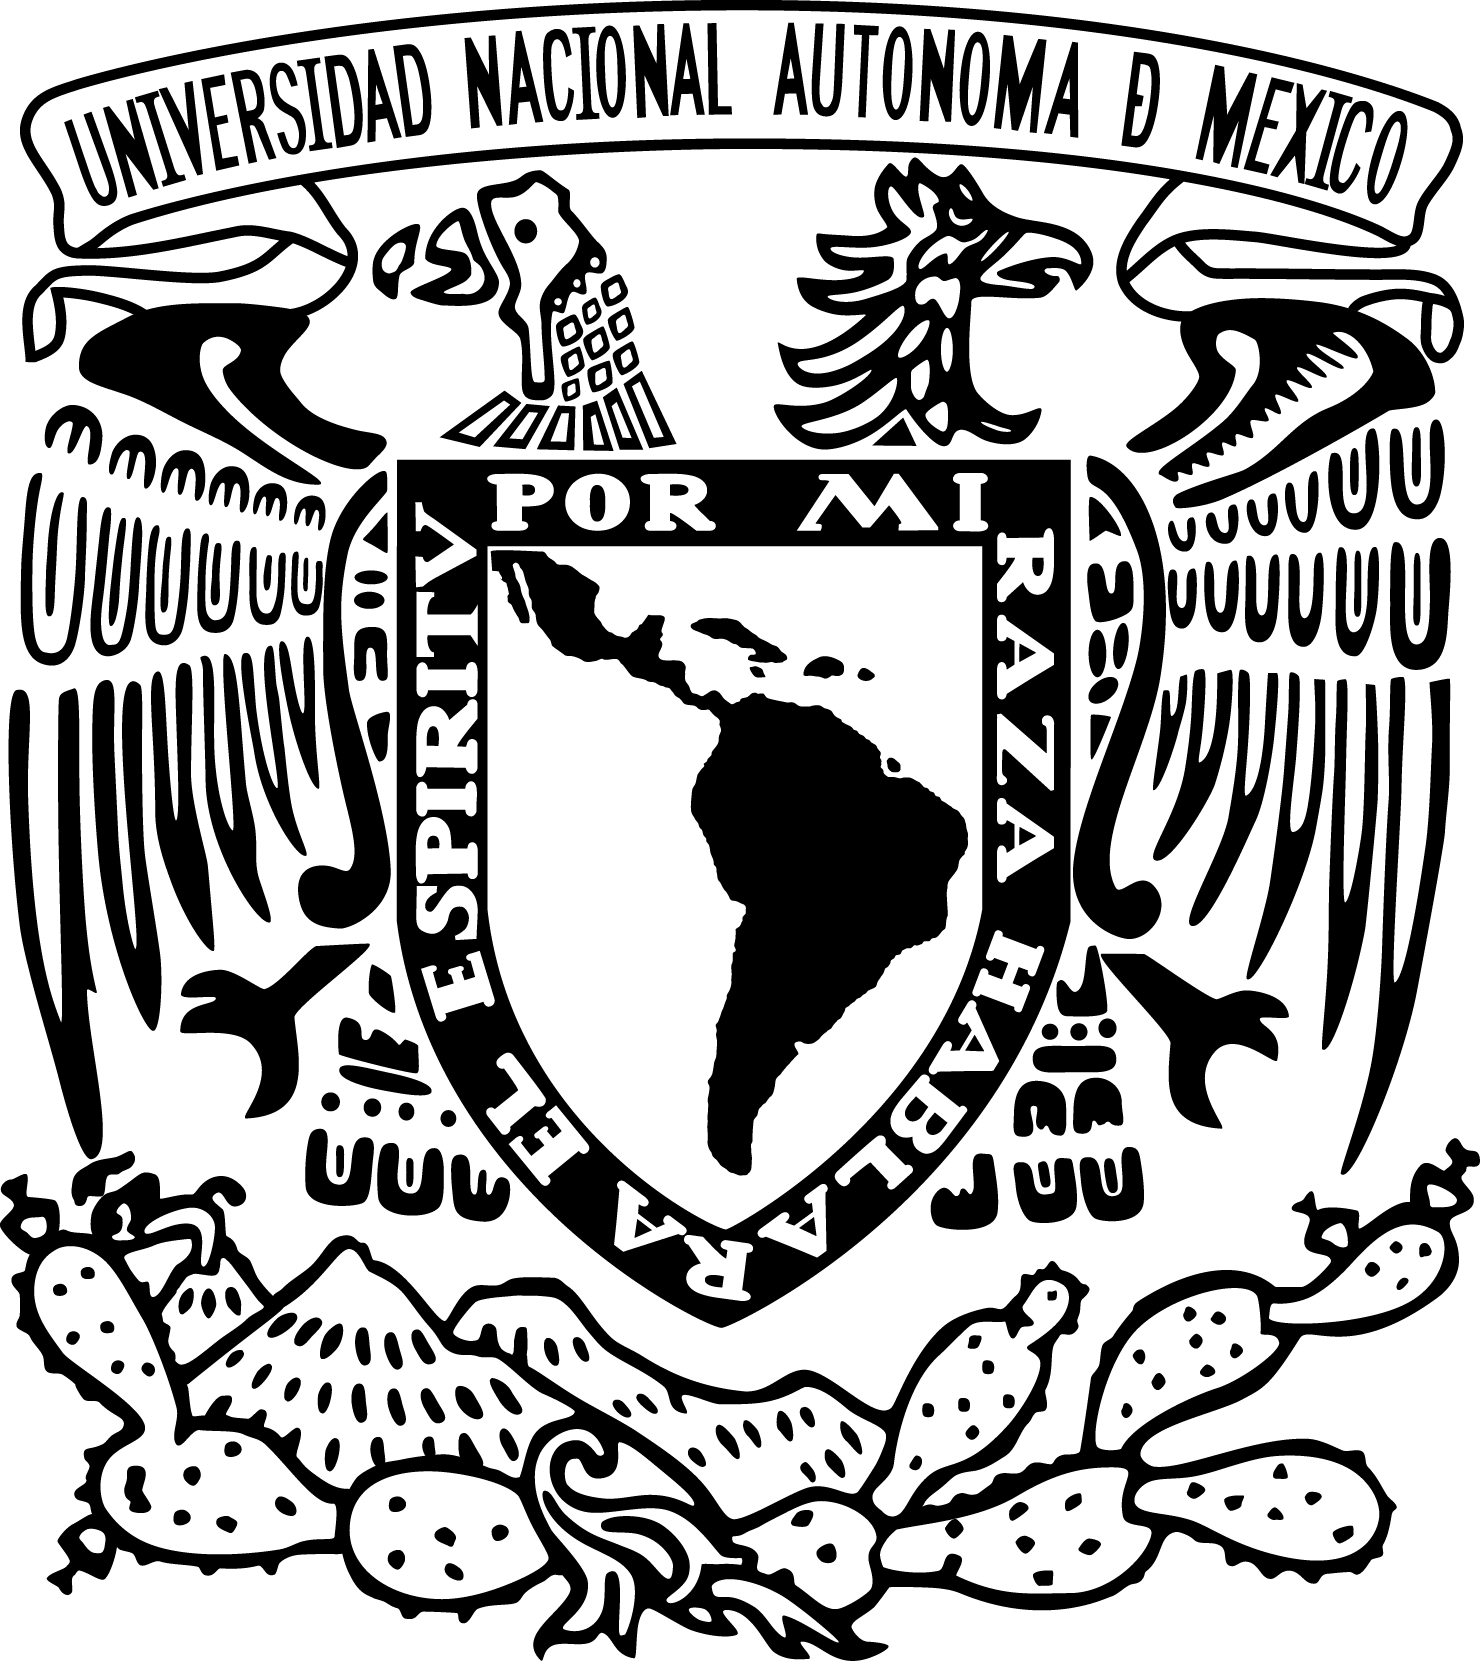
\includegraphics[height=1.5cm]{unam-escudo.png}}

\logo{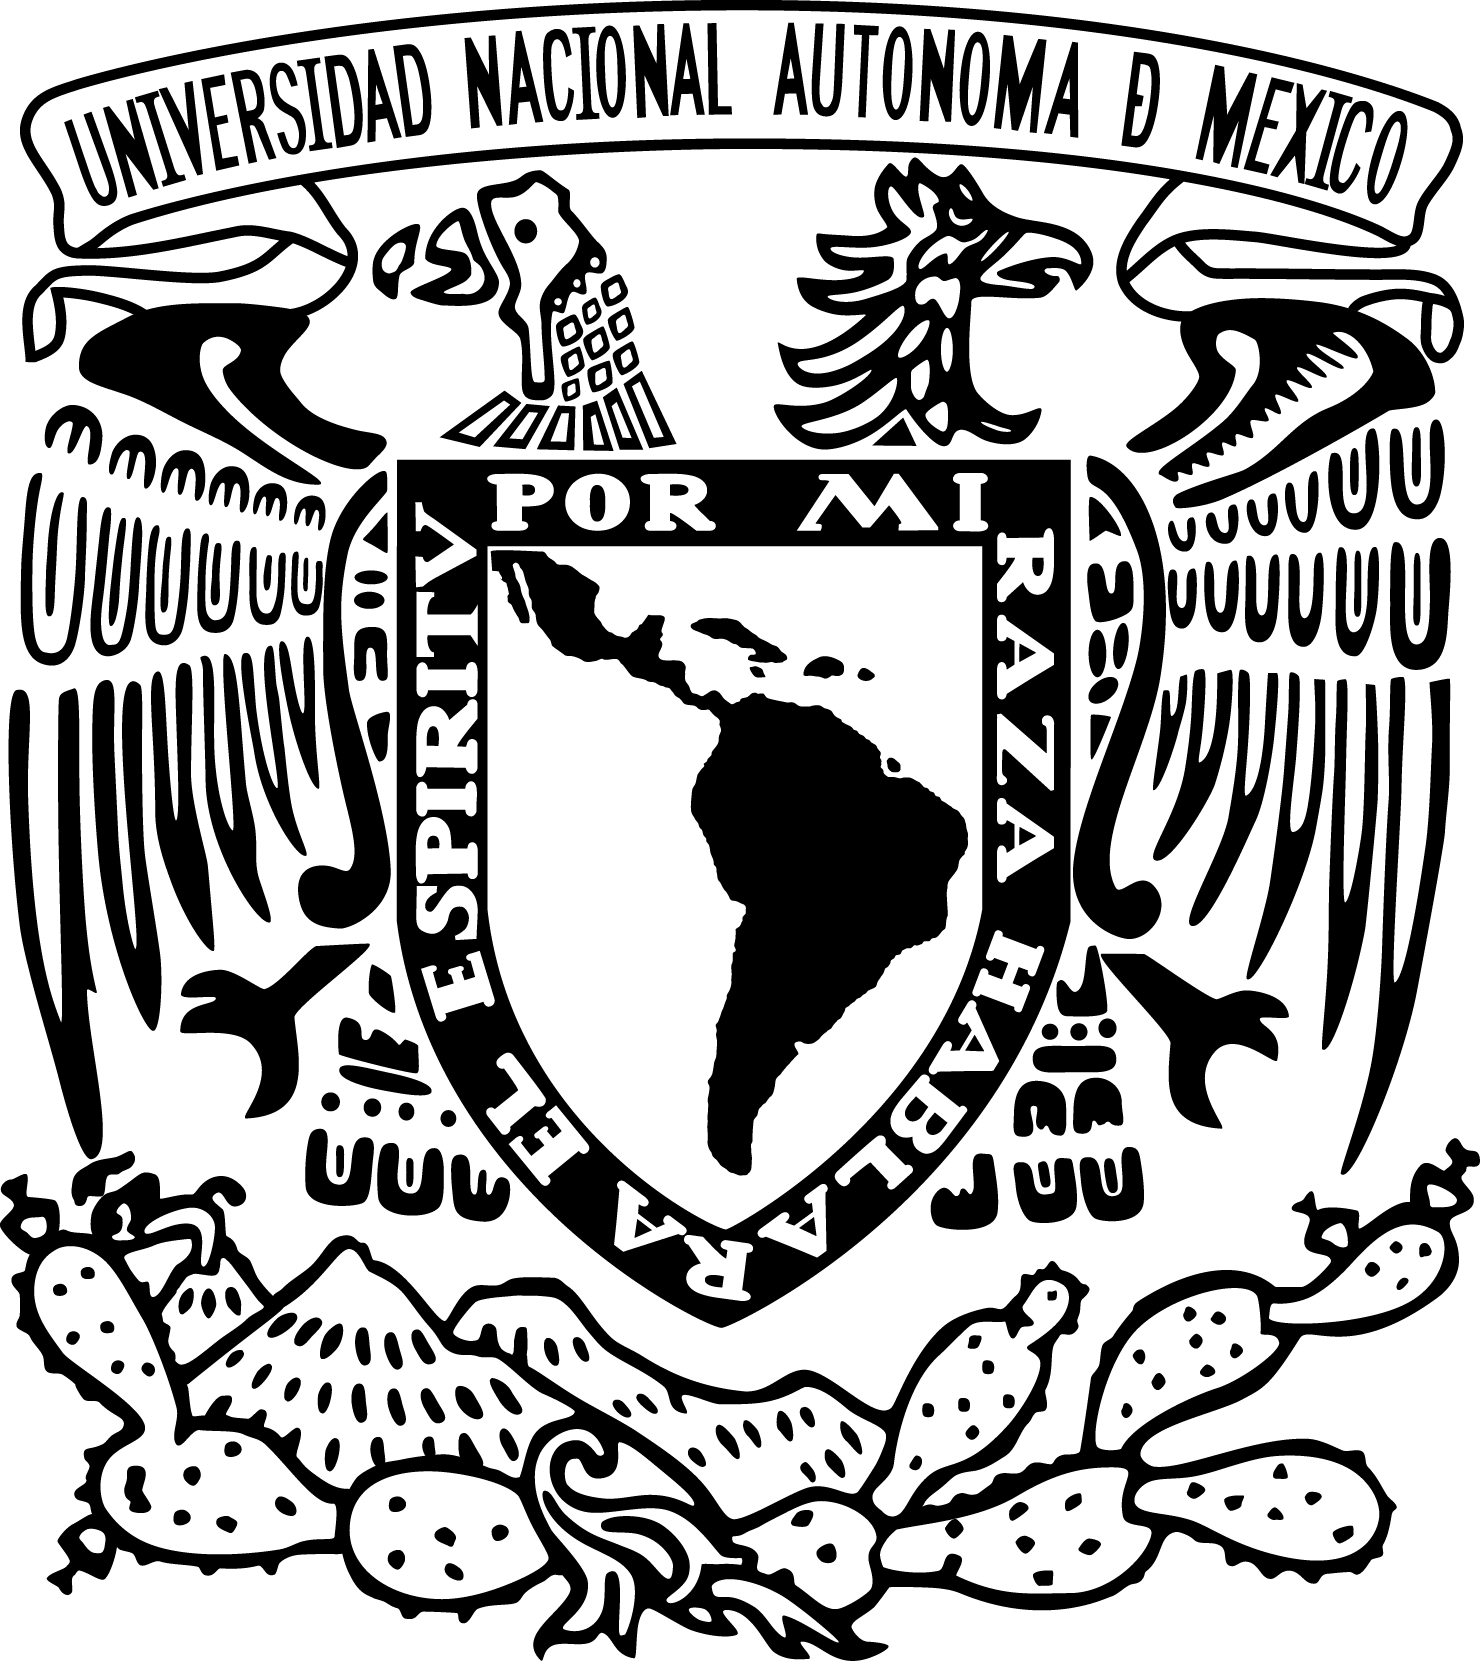
\includegraphics[height=0.8cm]{unam-escudo.png}\hspace{12pt}\vspace{-6pt}}
%\hspace{11cm}\vspace{-25pt}}  
      
\begin{document}

\maketitle

\begin{frame}{Contenido}
  \setbeamertemplate{section in toc}[sections numbered]
  \tableofcontents[hideallsubsections]
\end{frame}

\section{Introducción}

\begin{frame}{Sistemas complejos}

	\begin{itemize}
	\item<1->[$\blacksquare$]Los \textbf{sistemas complejos} conformados por una gran cantidad de componentes interactuando entre sí. 
	\item<2->[$\blacksquare$]George Zipf~\cite{zipf} trató a los idiomas como sistemas complejos.
	\only<2>{$$ f(k)\sim \frac{1}{k} $$}
	
	\item<3->[$\blacksquare$]Actualmente es evidente la influencia y el empleo de palabras inglesas.
	
	\item<4>[$\blacksquare$]Necesitamos una forma para entender cómo se mezclan los idiomas y cúal es la infuencia entre ellos.
	
	\end{itemize}

\end{frame}

\begin{frame}[fragile]{Objetivos}
	\begin{enumerate}
		\item Determinar la influencia de una lengua en otra a través de las palabras publicadas en los libros.
		\item Estimar las causas del movimiento de palabras entre idiomas a partir de sucesos históricos y culturales. 
	\end{enumerate}
\end{frame}


\begin{frame}[fragile]{Base de datos}
	
	\begin{itemize}
		\only<1-2>{\item[$\blacksquare$]Las publicaciones en los idiomas inglés, francés, alemán, italiano y español, en 269 años (1740-2009) obtenidas de Google Books \cite{ngramv}.}
		\vspace{1cm}
		\only<2>{\item[$\blacksquare$]Por cada año y por cada idioma se tomaron las 5 mil palabras mas usadas.}
		%\item<3>[$\blacksquare$]Cada palabra esta asociada a una frecuencia y un rango.	
	\end{itemize}
	
	\only<3>{	
		\begin{columns}
			\column[t]{4cm}    %new code
			\begin{itemize}
				\vspace{1cm}
				\item[$\blacksquare$]Cada palabra esta asociada a una frecuencia $f$ y un rango $k$.	
			\end{itemize}
			
			\column[t]{.5\textwidth}    %new code
			\begin{exampleblock}{Estructura de una lista}
				\begin{tabular}{ccc}
					\multicolumn{3}{c}{\textbf{Año $t$}}          \\
					Rango $k$     & Palabra    & Frecuencia $f$    \\
					1             & pal 1      & $f_{1}$            \\
					2             & pal 2      & $f_{2}$             \\
					3             & pal 3      & $f_{3}$              \\
					$\vdots$      & $\vdots$   & $\vdots$         \\
					$\vdots$      & $\vdots$   & $\vdots$         \\
					$5000$        & pal $5000$ & $f_{5000}$          
				\end{tabular}
			\end{exampleblock}
			
		\end{columns}
	}
\end{frame}

\begin{frame}[fragile]{Definiciones y forma de búsqueda}
	\begin{itemize}
		\item[$\blacksquare$]Las \textbf{palabras migrantes} son palabras que están presentes en al menos dos idiomas y con igual escritura, carácter por carácter.
		\item[$\blacksquare$]El \textbf{idioma origen} es aquel donde proviene la palabra migrante, y donde tiene un menor rango.
		\item[$\blacksquare$]El \textbf{idioma receptor} es aquel donde la palabra esta presente.		
	\end{itemize}	
\end{frame}

\begin{frame}[fragile]{Limpieza de datos e inconvenientes.}
	\begin{columns}
		\column[t]{.5\textwidth} 
		\only<1->{Se descartan:}
		\begin{itemize}
			\item<1->[$\blacksquare$] Palabras de contenido. Quedando sólo palabras funcionales.
			\item<2->[$\blacksquare$] Palabras combinadas con carácteres numéricos.
			\\
			\centering\textcolor{Sepia}{\textit{pag177}}
			\item<3->[$\blacksquare$] Palabras que aparecen sólo una vez en el idioma receptor.
			
		\end{itemize}
		
		\column[t]{.5\textwidth} 
		\only<4->{Algunas desventajas:}
		\begin{itemize}
			\item<4-6>[$\blacksquare$] No se distinguen plurales de singulares  ni conjugaciones verbales.
			\\
			\centering\textcolor{Sepia}{\textit{niño, niños, niña}}
			\item<5-6>[$\blacksquare$]Se encuentras palabras con diferentes significados pero igual escritura.
			\\
			\centering\textcolor{Sepia}{\textit{mayor}}
			\item<6>[$\blacksquare$]Define un origen distinto al verdadero.
			\\
			\centering\textcolor{Sepia}{\textit{natural}}
			
		\end{itemize}
		
	\end{columns}
\end{frame}

\section{Préstamos Nuevos}


\begin{frame}[fragile]{Definición y campos semánticos.}
	
	Los \textbf{préstamos nuevos} son palabras que aparecen por primera vez en las cinco mil más usadas del idioma receptor.
	
	Un \textbf{campo semántico} es un conjunto de palabras asociadas que comparten parte de su significado. 
\end{frame}

\begin{frame}
	\only<1>{
		\begin{columns}
			\column[t]{.5\textwidth}
			\begin{figure}[h!]
				\centering
				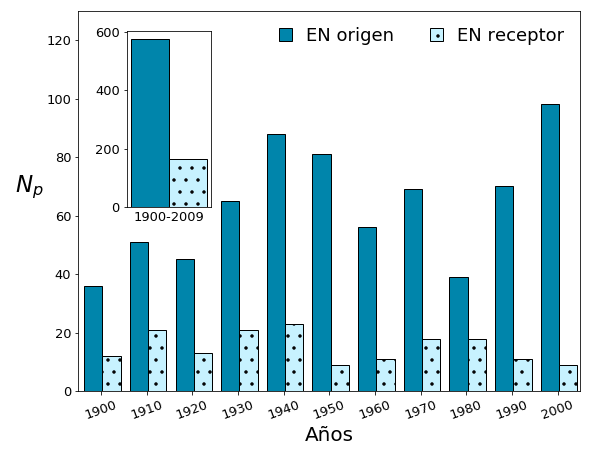
\includegraphics[width=\columnwidth]{BOR_EN.png}
			\end{figure}
			
			\column[t]{.5\textwidth} 
			\\
			\textcolor{Sepia}{Segunda Guerra Mundial.}
			\begin{itemize}
				\item churchill, catastrophe (1940)  
			\end{itemize} 
			
			\textcolor{Sepia}{Tecnología}
			\begin{itemize}
				\item internet, online, mail, software (1990 y 2000)
			\end{itemize}
			
			\textcolor{Sepia}{Globalización}
			\begin{itemize}
				\item standars, market, value, customer (1980, 1900, 2000)
			\end{itemize}
			
		\end{columns}
	}
	
	
	\only<2>{
		\begin{columns}
			\column[t]{.5\textwidth}
			\begin{figure}[h!]
				\centering
				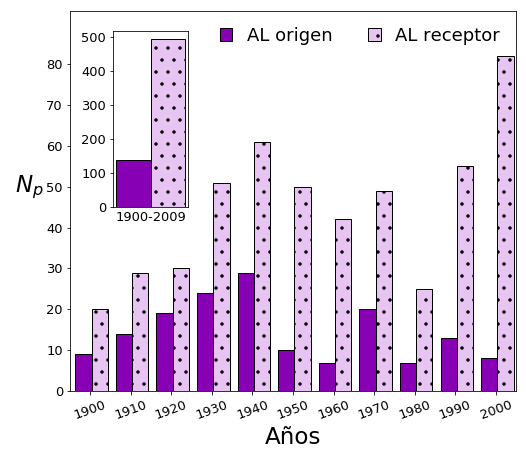
\includegraphics[width=\columnwidth]{BOR_GE.png}
			\end{figure}
			
			\column[t]{.5\textwidth} 
			\\
			\textcolor{Sepia}{Segunda Guerra Mundial.}
			\begin{itemize}
				\item lenin, hitler, reich, regierung, kaiser (1930, 1940)  
			\end{itemize} 
			
			\textcolor{Sepia}{Apellidos académicos.}
			\begin{itemize}
				\item beethoven, marx, freud, nietzsche,  engels, heidegger, hegel (1900-2000)
			\end{itemize}
			
		\end{columns}
	}	
	
	\only<3>{
		\begin{columns}
			\column[t]{.5\textwidth}
			\begin{figure}[h!]
				\centering
				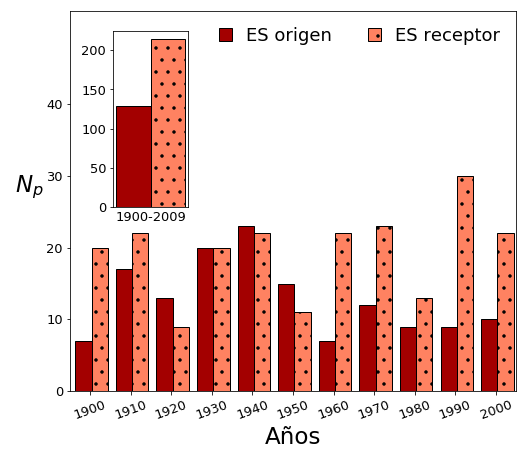
\includegraphics[width=\columnwidth]{BOR_SP.png}
			\end{figure}
			
			\column[t]{.5\textwidth} 
			\\
			\textcolor{Sepia}{Paises y ciudades de Latinoamérica.}
			\begin{itemize}
				\item chile, argentina, panama, buenos, aires (1900, 1910, 1940)  
			\end{itemize} 
			
			\textcolor{Sepia}{Medicina}
			\begin{itemize}
				\item virus, anemia, lepra, endovenosa, anestesia (1990, 1920, 1930, 1940)
			\end{itemize}
			
		\end{columns}
	}		
	

	
\end{frame}

\begin{frame}[fragile]{Resultados de los préstamos nuevos}
	\begin{itemize}
		\item [$\blacksquare$] Para haber una migración de palabras, debe ocurrir un evento histórico o cultural.\\
		
		\item [$\blacksquare$] Se logra decir las áreas donde los idiomas son más influyentes.
		\begin{itemize}
			\item Inglés: guerra, política, tecnología y globalización.
			\item Francés: guerra política y apellidos académicos.
			\item Alemán: guerra y apellidos académicos.
			\item Italiano: guerra e ideologías políticas.
			\item Español: medicina y nombres de países Latinoamericanos. 
		\end{itemize}
	\end{itemize}
\end{frame}


\section{Préstamos Acumulados}



\begin{frame}[fragile]{Características}
	
	\visible<1->{$\blacksquare$ Un \textbf{préstamo acumulado} es una palabra con origen $A$ que ya habia aparecido en $B$, y para un determinado año lo vuelve a hacer.}
	
	\visible<2->{$\blacksquare$ Los préstamos nuevos se vuelven acumulados si aparecen posterior a su año de migración.}
	
	\visible<3>{
		\centering
		\begin{tabular}{lcccccc}
			\multicolumn{7}{c}{R E C E P T O R}                                                                                                                                             \\
			\multirow{6}{*}{\begin{tabular}[c]{@{}l@{}}O\\ R\\ \,I\\ G\\ E\\ N\end{tabular}} &             & \textbf{inglés} & \textbf{francés} & \textbf{alemán} & \textbf{italiano} & \textbf{español} \\
			& \textbf{inglés}   & -           & 6.48$\%$  & 3.28$\%$      & 1.55$\%$   & 1.47$\%$    \\
			& \textbf{francés}  & 5.94$\%$    & -         & 1.88$\%$      & 2.37$\%$   & 1.32$\%$    \\
			& \textbf{alemán}   & 1.27$\%$    & 1.28$\%$  & -             & 0.69$\%$   & 0.30$\%$    \\
			& \textbf{italiano} & 1.55$\%$    & 2.01$\%$  & 0.95$\%$      & -          & 4.38$\%$    \\
			& \textbf{español} & 2.36$\%$     & 1.68$\%$  & 0.50$\%$      & 6.23$\%$    & -          
		\end{tabular}
	}
	
\end{frame}

\begin{frame}[Fragile]{El uso entre idiomas.}
	Dados un origen $A$ y un receptor $B$:
	\begin{enumerate}
		\item<1-> Sumamos las frecuencias de las 5 mil palabras de B.
		$$\sum_{k=1}^{5000} f(k)$$
		
		\item<2-> Localizamos y sumamos las frecuencias de los prestamos acumulados de A.
		$$\sum_{j} f(j) $$
		
		\item<3->Obtenemos el \textbf{uso} al dividir las dos cantidades
		\begin{equation}
		\label{ec.fuso1}
		\underset{ \text{\tiny A} \to  \text{\tiny B} }{U}(t) = \frac{\sum_{j} f(j)}{\sum_{k=1}^{5000} f(k)}.
		\end{equation}	
	\end{enumerate}
	
	
\end{frame}

\begin{frame}
	\only<1->{
		\begin{center}
			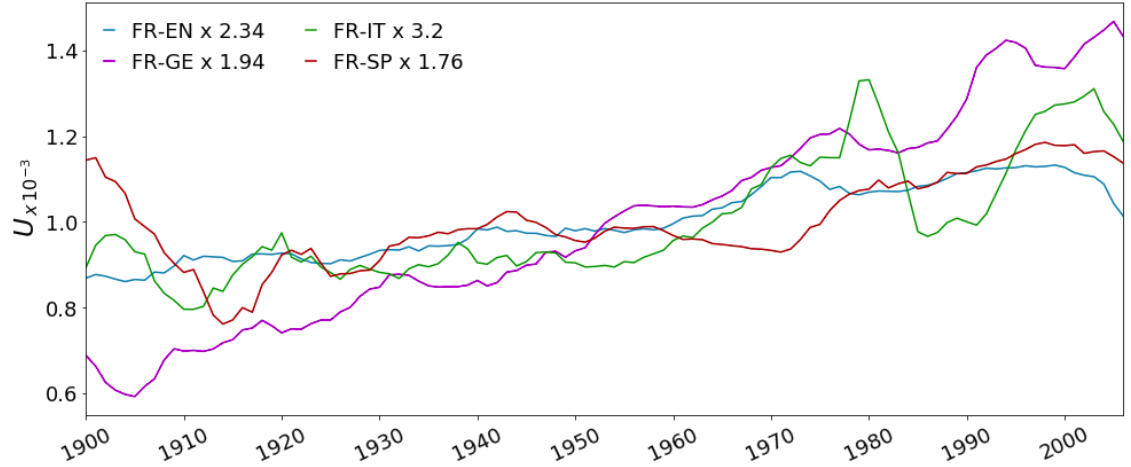
\includegraphics[height=4.5cm]{FR_UOR.png}
		\end{center}
		}
		
		\only<1>{ $$fpa =\frac{\Delta U}{\Delta t}$$}
		
		\only<2->{Mayor Uso: Italiano 0.0031 fpa (1950-1970) y español 0.0015 fpa (1970-1995).
	}
	\\
	\only<3>{\textcolor{Sepia}{Revolución Francesa}
		\begin{itemize}
			\item bastille, bourgeois, napoleon, imperiale 
		\end{itemize}
	}
	\only<4>{\textcolor{Sepia}{Religión}
		\begin{itemize}
			\item saint, eglise, dime
		\end{itemize}
	}
	\only<5>{\textcolor{Sepia}{Industria vitivinícola}
		\begin{itemize}
			\item raisins, vin, vignoble, recolte.
		\end{itemize}
	}
	
\end{frame}
%{
%\begin{frame}
%	\only<1->{
%		\begin{center}
%			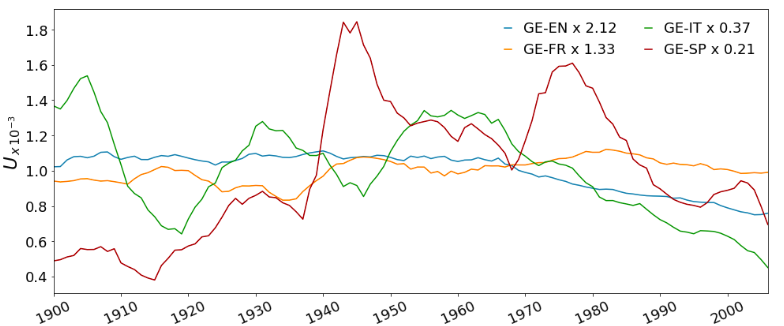
\includegraphics[height=4.5cm]{GE_UOR.png}
%		\end{center}
%		
%		Mayor Uso: Español 0.0021 fpa (1935-1945),  inglés -0.00015 (1960-2009).
%	}
%	\\
%	\only<2>{\textcolor{Sepia}{Segunda Guerra Mundial.}
%		\begin{itemize}
%			\item berlin, hitler, reich, testen.
%		\end{itemize}
%	}
%	\only<3>{\textcolor{Sepia}{Apellidos académicos}
%		\begin{itemize}
%			\item marz, freud, heideggger, nietzsche, hegel, engels. 
%		\end{itemize}
%	}
	
%\end{frame}

\begin{frame}
	\only<1->{
		\begin{center}
			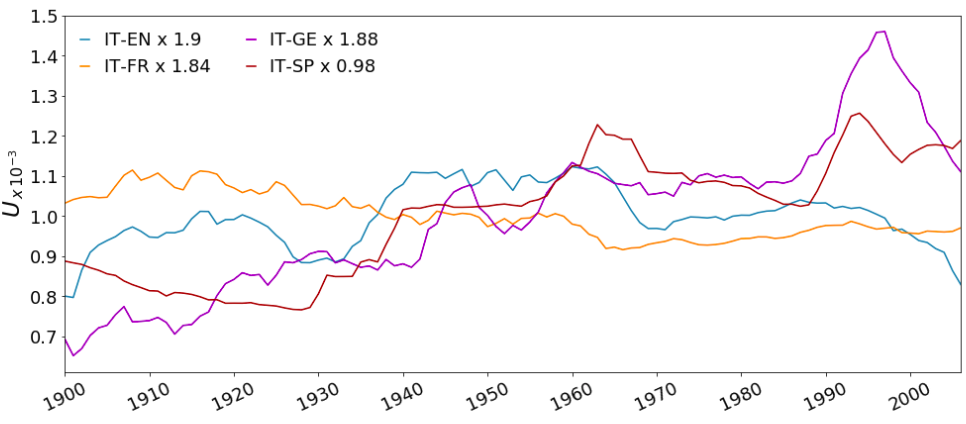
\includegraphics[height=4.5cm]{IT_UOR.png}
		\end{center}
		
		Mayor Uso: Inglés 0.0035 fpa (1930-1940), español 0.0011 fpa (1930-1960).
	}
	\\
	\only<2>{\textcolor{Sepia}{Segunda Guerra Mundial.}
		\begin{itemize}
			\item mussolini, fascismo, battlagia.
		\end{itemize}
	}
	\only<3>{\textcolor{Sepia}{Religión}
		\begin{itemize}
			\item santo, suora, cattedrale. 
		\end{itemize}
	}
	
\end{frame}

\begin{frame}{Resultados sobre los préstamos acumulados}
	\begin{itemize}
		\item [$\blacksquare$]  El idioma más utilizado, no es siempre el que tiene más préstamos acumulados.
		\item [$\blacksquare$] Si el uso aumenta en los años alrededor de un suceso, las palabras de un campo semántico aumentarán su frecuencia.
		\item [$\blacksquare$] Obtenemos una base del contenido que ha conformado a un idioma.
	\end{itemize}
\end{frame}

\section{Robustez} 

\begin{frame}[fragile]{Eliminación y similitud}
	\only<1->{
	Problemas :}
	\begin{itemize}
		\item <2->No sabemos detectar de forma práctica los errores.
		\item <3->Tampoco conocemos como afecta una posible limpieza al uso entre idiomas.
	\end{itemize}
	
	\only<4->{
	Solución:}
	\begin{itemize}
		\item <4->Eliminar préstamos acumulados y ver la similitud entre el uso original y el reducido.
		$$
		\left\langle D \right\rangle  = \frac{1}{N}\sum_{t=1}^{N} \left| u_{t} - r_{t} \right|.
		$$
		\item <5>Controlar el tamaño de la eliminación. 
	\end{itemize}
\end{frame}

\begin{frame}{Resultados previos}
	\begin{itemize}
	\item<1-> [$\blacksquare$]  Eliminabamos palabras al azar sin importar su rango.
	\end{itemize}
	\visible<2->{
	\begin{center}
			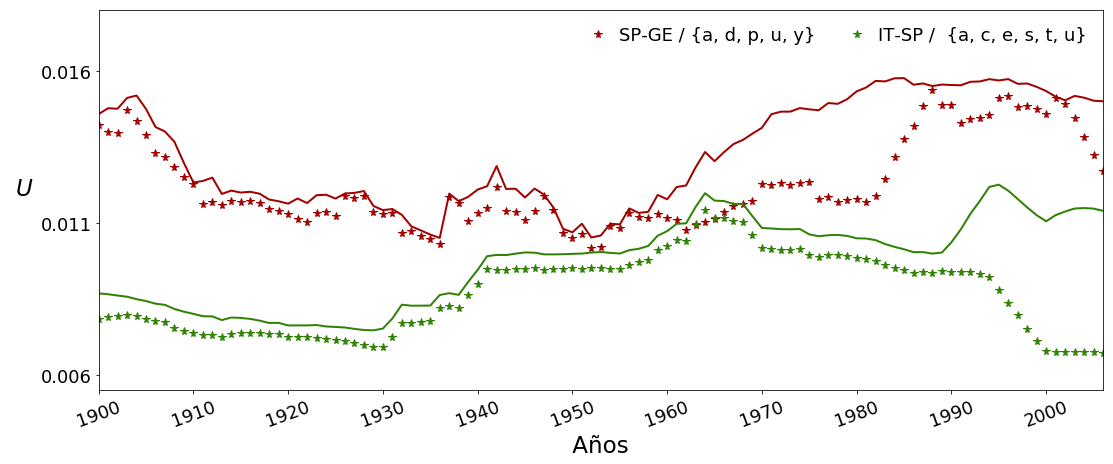
\includegraphics[height=4.5cm]{OM2.png}
		\end{center}
		}
	\begin{itemize}
	\item<3-> [$\blacksquare$] Podiamos eliminar muchas palabras sin afectar la similitud.
	\end{itemize}
\end{frame}

\begin{frame}{Nuevos Resultados}
	\begin{itemize}
		\item<1->[$\blacksquare$] Eliminando palabras en los rangos bajos.
	\end{itemize}
	\visible<2->{
	\begin{figure}[h!]
		\centering
		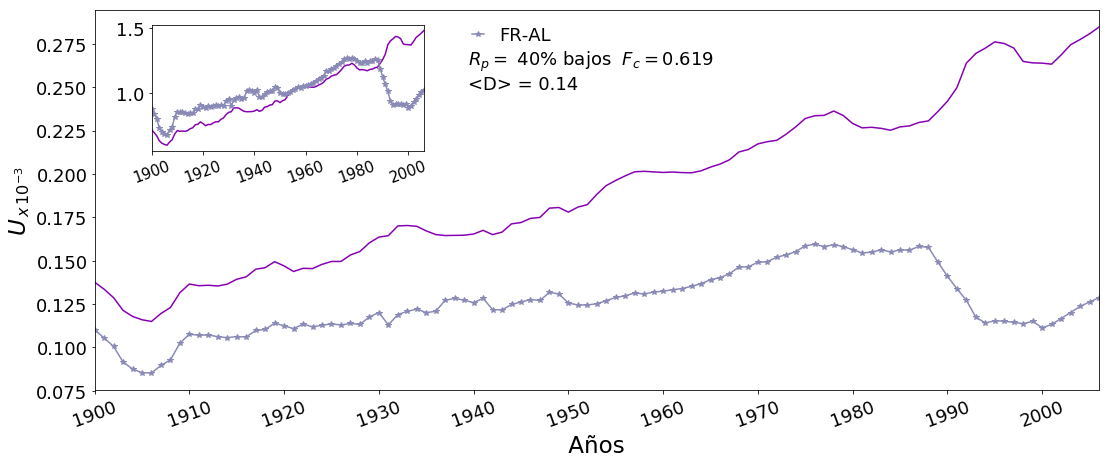
\includegraphics[height=3.2cm]{OM_FG1.png}
	\end{figure}
	}
	
    \hrule
    
	\begin{itemize}
		\item<3->[$\blacksquare$] Eliminando palabras en los rangos altos.
	\end{itemize}
	\visible<4>{
	\begin{figure}[h!]
		\centering
		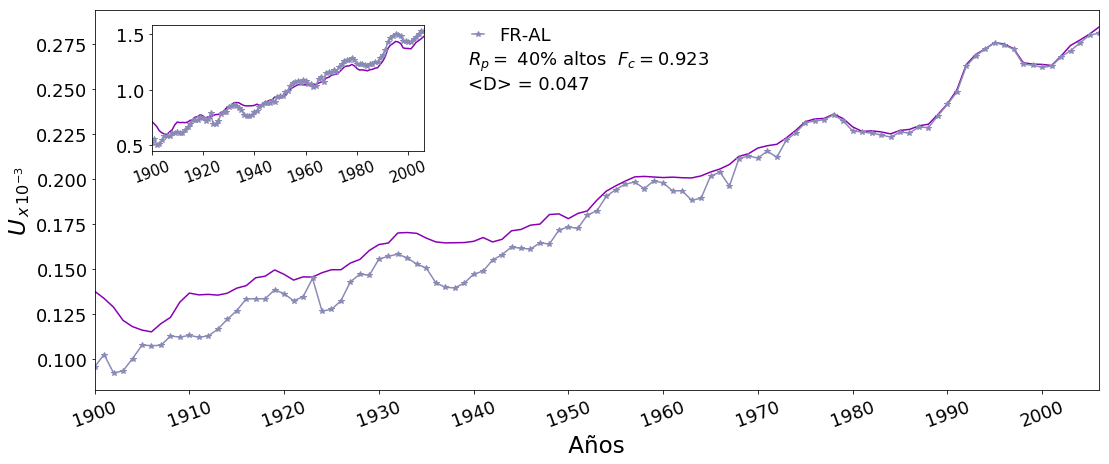
\includegraphics[height=3.2cm]{OM_FG2.png}
	\end{figure}
	}
\end{frame}


\begin{frame}{¿Qué tanto podemos eliminar?}

\begin{columns}
	\column[t]{.5\textwidth}
	\visible<1->{
	Rangos bajos 
	\begin{figure}[t]
		\centering
		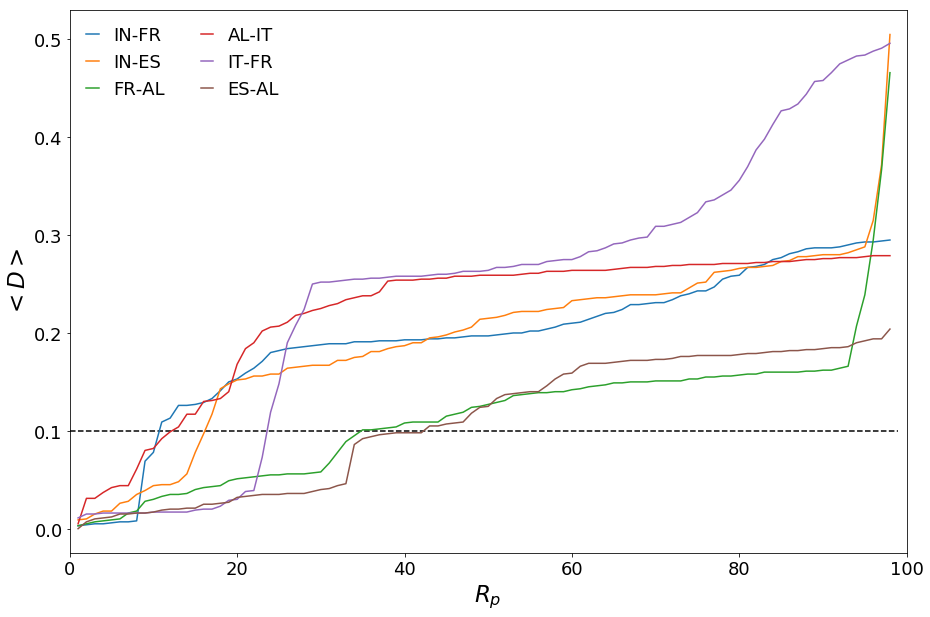
\includegraphics[width=5.2cm, height=4.2cm]{OM_bajos.png}
	\end{figure}
	}

	\column[t]{.5\textwidth}
	\visible<2->{
	Rangos altos 
	\begin{figure}[t]
		\centering
		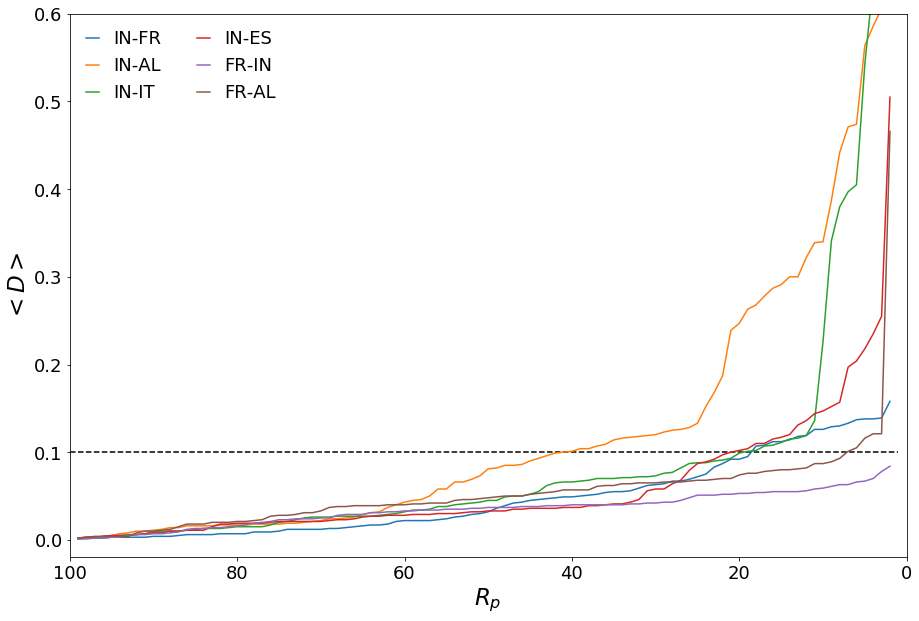
\includegraphics[width=5.2cm, height=4.2cm]{OM_altos.png}
	\end{figure}
	}
\end{columns}

\visible<3->{
	\begin{itemize}
	\item<3-> [$\blacksquare$]El peso del uso entre idiomas lo llevan las palabras con los rangos bajos. 
	\item<4-> [$\blacksquare$]Nuestro algoritmo es bueno si en las palabras más frecuentes hay pocos errores en la clasificación.
	\end{itemize}
	}

\end{frame}

\section{Diversidad de rango}

\begin{frame}{Motivación}
	\begin{itemize}
	\item<1->[$\blacksquare$] ¿Cómo estan cambiando las palabras más frecuentes, si estas son las que llevan el peso del uso?
	\item<2->[$\blacksquare$] ¿Que tanto modifican su rango los préstamos acumulados?
	\end{itemize}
	
	\\
	\vspace{5mm}
	\only<3->{
	La diversidad de rango $d(k)$ es el cociente entre la cantidad de palabras que ocupan un mismo rango $k$, en un mismo intervalo de tiempo $\Delta t$. 
	}
	
\end{frame}

\begin{frame}{Dos formas de ajustar los resultados}

\only<1-3>{
\begin{figure}[t]
	\centering
	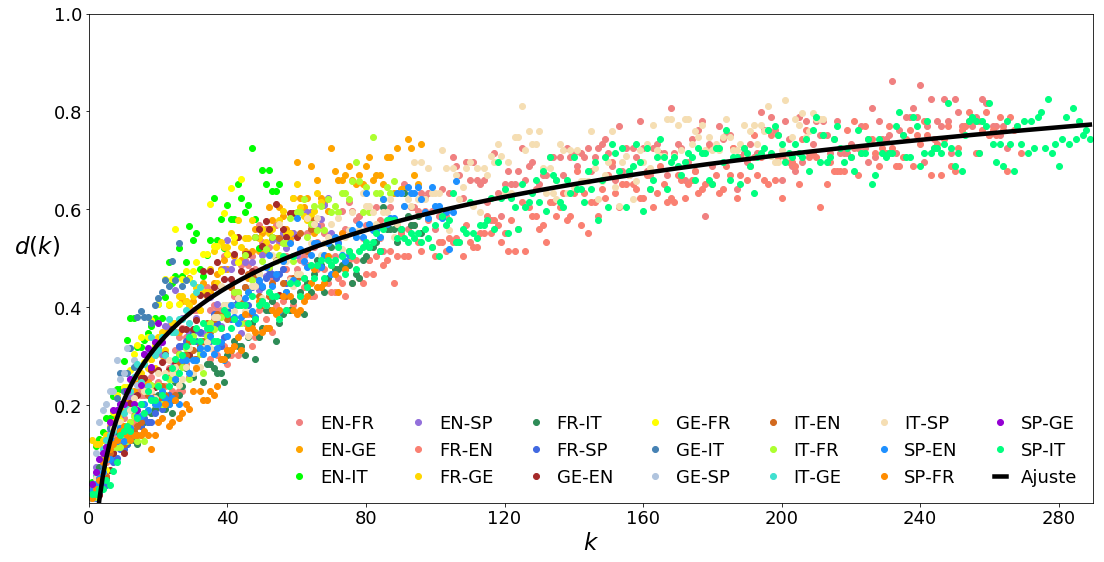
\includegraphics[height=4.5cm]{DR_gen.png}
\end{figure}

\begin{equation}
	\label{ec.dklog}
	d(k) = 0.16\ln(k) - 0.17.
\end{equation}

\begin{itemize}
\item<2->[$\blacksquare$] Facíl de calcular.
\item<3>[$\blacksquare$] No es fiable para combinaciones con pocos rangos.            $R^{2} = \left [0.79, 0.95  \right ]$.
\end{itemize}
}

\only<4->{
\begin{figure}[t]
	\centering
	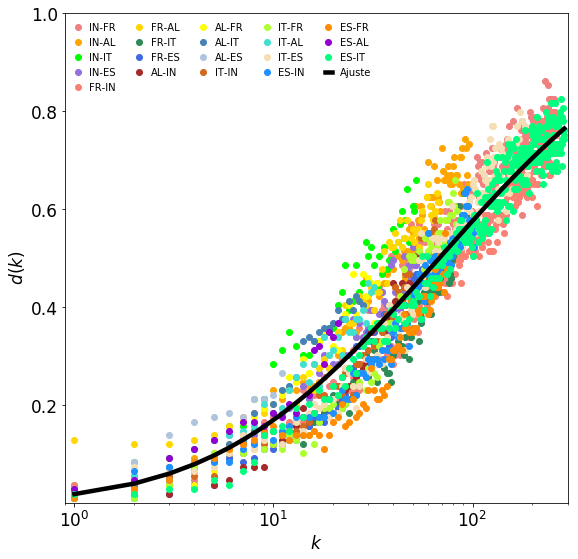
\includegraphics[height=4.5cm, width =4.5cm]{DR_sig.png}
\end{figure}
\only<4-6>{
\begin{equation}
	\label{ec.dksig}
	d(k) = \frac{1}{\sigma\sqrt{2\pi}}\int_{-\infty }^{\log_{10^{k}}} e^{-\frac{\left ( y-\mu \right )^{2}}{2\sigma^{2}}}dy.\,\,\,\,\,\,\,\, \mu = 1.83\,\,\sigma = 0.87
\end{equation}
}

\only<5-6>{
\begin{itemize}
\item<5-6>[$\blacksquare$] Fiable sin importar la cantidad de rangos, en promedio $R^{2}=0.95$.
\item<6>[$\blacksquare$] Concuerda con los resultados previos  de~\cite{iplosone}hechos támbien sobre idiomas, y sobre deportes y juegos~\cite{epj}.
\end{itemize}
}
}

\only<7->{
Sobre la diversidad :
\begin{itemize}
\item<7->[$\blacksquare$] Las palabras más cambiantes son las que tienen rangos medios y altos. 
\item<8> [$\blacksquare$] El comportamiento  es valido sin importar el tamaño del corpus.
\end{itemize}
}
\end{frame}

\section{Conclusiones}

\begin{frame}
\only<1-4>{
	\begin{itemize}
	\item<1->[$\blacksquare$] Las migraciones y el aumento del uso  entre idiomas son provocadas por eventos historicos o culturales.
	%\item<2-4>[$\blacksquare$] El suceso tambien  hará que las palabras de su campo semantico aumenten su frecuencia.
	\item<2->[$\blacksquare$] Los idiomas influyen más que otros en ciertas areas.
	\item<3->[$\blacksquare$] Los errores en las clasificaciones pueden ser  despreciables si estos estan en los rangos más altos. 
	\item<4>[$\blacksquare$] A lo largo del tiempo, las palabras que modifican más su rango, están en los rangos medios y altos. 
	\end{itemize}
	}
		
	\only<5>{
	\begin{itemize}
	\item<5> Inglés: politica, tecnología y globalización.
	\item<5> Francés: religión, industria vitivínicola  y apellidos académicos.
	\item<5> Alemán: guerra y apellidos académicos.
	\item<5> Italiano: guerra e ideologías políticas.
	\item<5> Español: medicina y nombres de países Latinoamericanos. 
	\end{itemize}
	}


\end{frame}


\begin{frame}[allowframebreaks]{Bibliografía}
%        \bibliographystyle{amsalpha}
\printbibliography
%        \bibliography{bib2.bib}
\end{frame}


\end{document}